\chapter{抗衰落技术}
\section{抗衰落}
\subsection{传输中的损耗}
\begin{itemize}
	\item 阴影效应 →通信范围
	\item 多径效应,多普勒效应。衰落 通信质量
	\item 噪声和干扰,误码。通信质量
\end{itemize}
\subsection{抗衰落措施
}
\begin{enumerate}
	\item 信道编码→减小信道噪声或干扰
	\item 扩频技术→减小多径干扰
	\item 分集→减小衰落深度和衰落持续时间
	\item OFDM(均衡技术)→减小码间干扰
	\item  MIMO(空间分集)→克服衰落,降低误码率
\end{enumerate}

\section{分集技术}
定义:接收端对它收到的多个衰落特性\textbf{互相独立(携带同一信息)}的信号进行\textbf{集中}处理,以降低信号电平起伏的办法。\\
{\centering \textbf{分散传输} \hspace{3cm} \textbf{集中处理}}
\subsection{分集技术的分类}
\begin{description}
	\item[宏分集“基站分集”] 将多个基站设置在不同的地理位置上和不同的方向上,移动台可和其中信号最好的一个基站进行通信。它能克服\textbf{由于阴影效应或地形影响而产生的慢衰落}\item[微分集] 在同一场地采用多副天线或多
	个频率或多种极化等方法接收和处理由多条路
	径传来的信号。移动台和基站都可使用这种技
	术。(空间、频率、极化、场分量、角度及时间),克服\textbf{快衰落}。
\end{description}
\subsubsection{空间分集}
原理:空间分集的依据在于快衰落的空间独立性。\\当两个位置的距离大于一定程度,则两处的信号衰落是不相关的。在频率较高时($ f \ge 800MHz$,容易实现空间分集。
\subsubsection{时间分集}
原理:同一信号在不同的时间区间多次重发,只要
各次发送的\textbf{时间间隔足够大},那么各次发送信号所出
现的衰落将是\textbf{彼此独立}的。\\
实现:其重发时间间隔 $\Delta T \ge \frac{1}{2fm} = \frac{1}{2(v/\lambda)}$,用于\textbf{克服多普勒效应引起的信号衰落现象}(所以移动台静止时,v=0,时间分集不起作用)。 
\subsubsection{频率分集}
原理:相干带宽之外的频率上不会出现同
样的衰落
实现:多个载频上传送信号,载频间隔大
于相干带宽$ B_c = \frac{1}{2\pi\Delta} $
\subsubsection{极化分集}
原理:两个不同极化的电磁波具有独立的衰
落特性。\\
实现:收发端用不同极化的天线分别发送和
接收信号,以获得分集效果。\\
极化分集是空间分集的一种特殊情况。将射频功率分给两个不同的极化天线,所以发射功率要损失3db。

\subsection{合并技术}
多路接受信号的加权求和。
\subsubsection{选择式合并SC}
在多路信号中选择信噪比最高的支路作为输出,即在多个加权系数中,只有一个伪1,其余为0.
\subsubsection{最大比值合并MRC}
最大壁纸合并将各路信号加权后合并。在信号合并前对各路载波相位进行调整使之同相,然后相加。\\
各路加权系数$ a_k $与信号包络$ r_k $成正比,于噪声$ N_k $成反比。这是\textbf{最佳的合并方式}。
\begin{equation}\label{key}
a_k = \frac{r_k}{N_k}
\end{equation}
所以合并信号为:
\begin{equation}\label{key}
r_R = \sum_{k=1}^{M}a_kr_k = \sum_{k=1}^{M}\frac{r_k^2}{N_k}
\end{equation}
\subsubsection{等增益合并EGC}
。无需对信号加权,
各支路的信号是等增益相加的。
\begin{equation}\label{key}
r_R = \sum_{k=1}^{M}r_k
\end{equation}
\subsection{合并技术性能分析于比较}
最大比值合并 > 等增益合并 > 选择式合并\\
合并增益D(M)与分集支路数目(M)
之间的关系:
\begin{figure}[H]
	\centering
	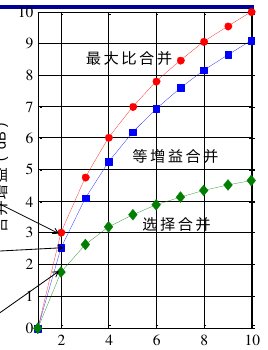
\includegraphics[width=0.7\linewidth]{figures/hebingbijiao.png}
	\caption{}
	\label{fig:}
\end{figure}
\section{信道编码技术}
\subsubsection{一些理论}
信道编码是为了保证信息传输的可靠性、提高传输质量而设计的一种编码。\\
通常分为\textbf{分组码}和\textbf{卷积码}。\\
\textbf{定义:} 在信息码元中增加一些冗余码元,用来在接收端
检测或纠正在有噪信道中引入的误码\\
码字:信息码元于冗余码元一起构成的消息块称为码字。\\
码距:对应位不同的个数,又称为汉明距。信道编码的实质就是\textbf{增加码距,码距代表了纠检错能力}\\
码距于纠检错能力的关系:
\begin{itemize}
	\item 检测e个错误:最小码距d0$\ge$e+1
	\item 纠正t个错误:最小码距d0$\ge$2t+1
	\item 纠正t个错误,发现e个码位错误:最小码距d0$\ge$t+e+1
\end{itemize}
\subsubsection{信道编码分类}
\begin{itemize}
	\item 按码组功能分:检错码和纠错码
	\item 按加入冗余码元方式:线性码和非线性码
	\item 按码组结构分:分组码和卷积码
	\item  按纠错能力分:纠随机错和纠突发错
	
\end{itemize}
性能指标:编码效率,编码增益,编码延时,编译码器的复杂度
\subsubsection{应用}
\begin{itemize}
	\item GSM,IS-95,卷积码
	\item 3G,卷积,Trobo
\end{itemize}
\subsubsection{线性分组码}
主要考虑CRC循环冗余校验,用于误码检测。表示为(n,k)码,k为输入,n为输出,编码效率R = k/n\\
生成方式:
\begin{figure}[H]
	\centering
	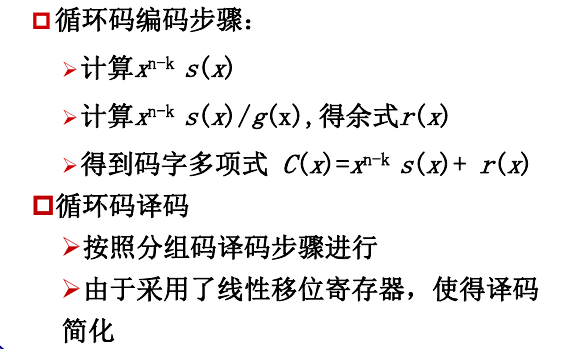
\includegraphics[width=0.7\linewidth]{CRCshengcheng.png}
	\caption{}
	\label{fig:crc}
\end{figure}
例题:
\begin{figure}[H]
	\centering
	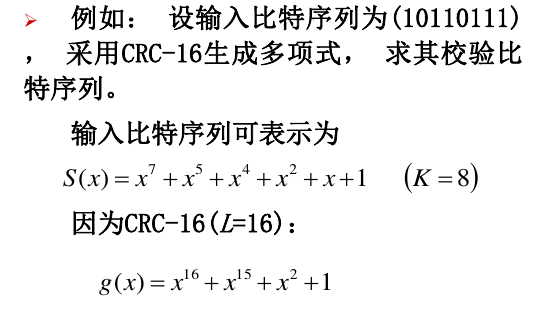
\includegraphics[width=0.7\linewidth]{CRC1.png}	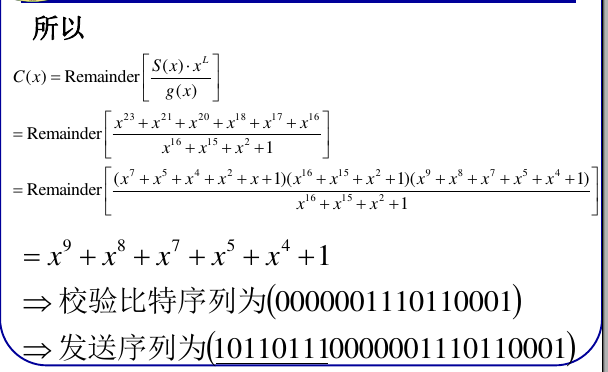
\includegraphics[width=0.7\linewidth]{CRC2.png}
	\caption{}
	\label{fig:crc1}
\end{figure}
\textbf{简便算法:}
\begin{figure}[H]
	\centering
	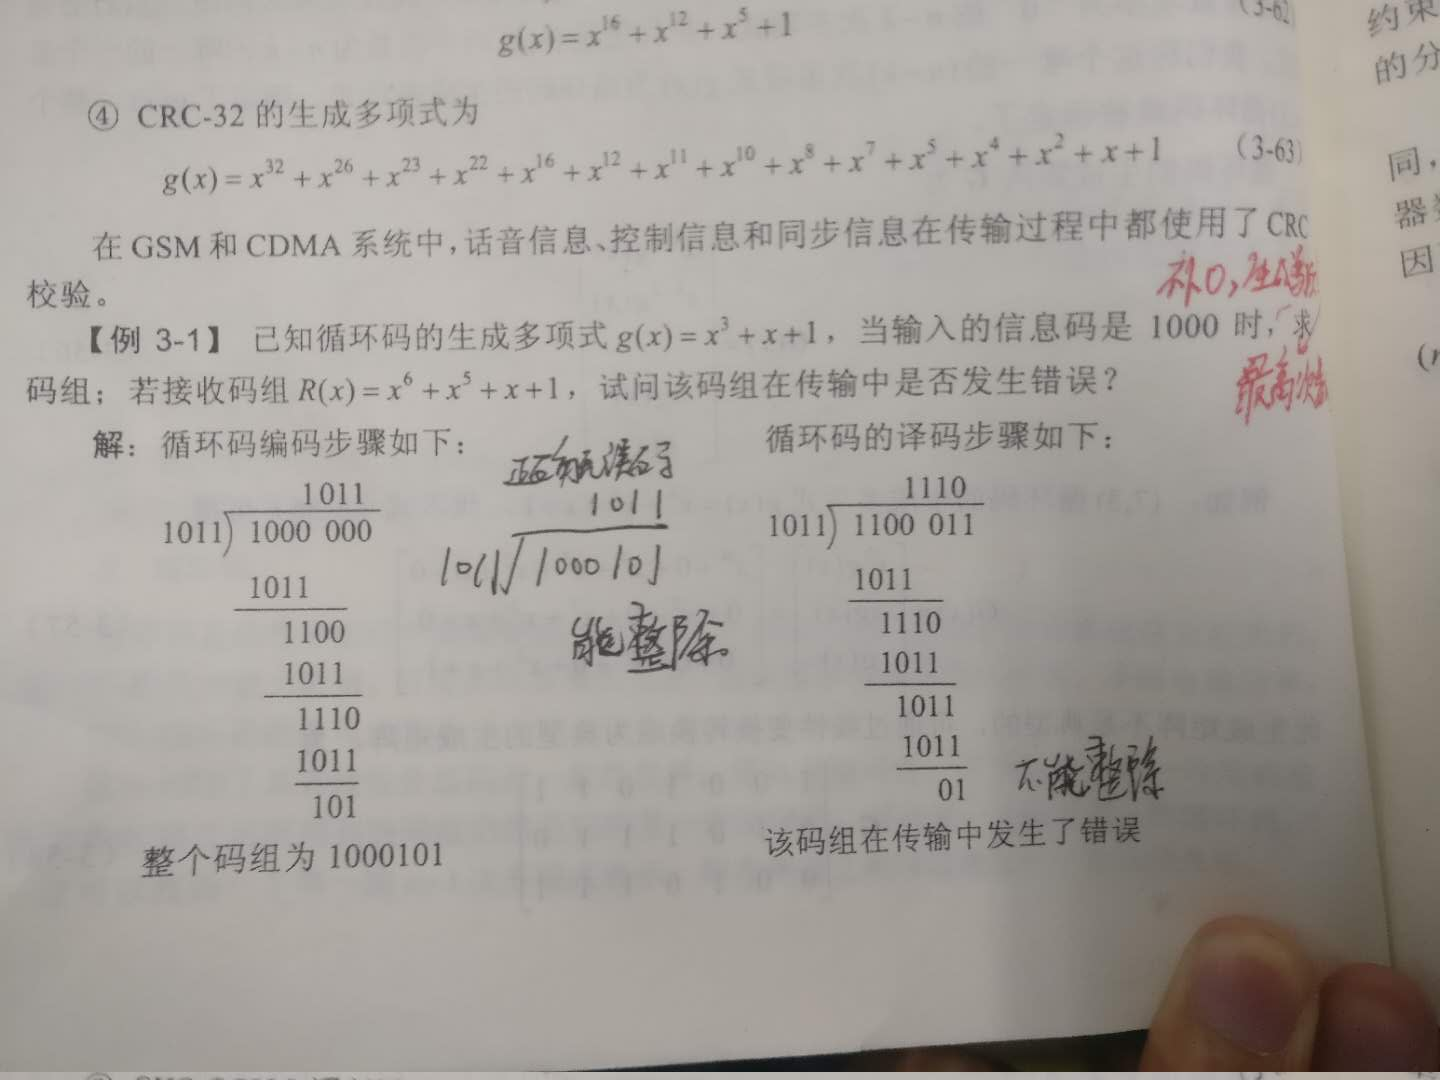
\includegraphics[width=0.7\linewidth,height=7cm]{CRC3.jpeg}
\end{figure}
验证是否出现误码,将接收到的序列除以生成多项式,整除则(可能)无误码,否则有误码。
\subsection{卷积码}
卷积码的监督码元与当前码元和前若干码
元有关。表示为(n,k,m),m为寄存器的个数。约束长度l = m+1,编码效率R=k/n。\\
为什么要称为卷积码?采用单位冲击信号输入后,得到各支路的冲激响应,将输入于各支路的冲击响应做卷积运算可得到各支路的信号输出。
\subsubsection{卷积码的描述}
\begin{enumerate}
	\item 解析法,离散卷积法、码生成多项式法、生成矩阵、
	\item 图形法,状态图、树图以及网格图
\end{enumerate}
\subsubsubsection{图解法}
\begin{description}
	\item[状态图] 圈内为寄存器状态,单斜杠前为输入,后为输出,箭头方向为寄存器转移方向。如:
	\begin{figure}[H]
		\centering
		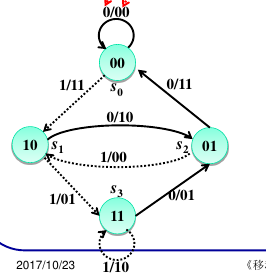
\includegraphics[width=0.7\linewidth]{zhuangtaizhuanyi.png}
		\caption{}
		\label{fig:}
	\end{figure}
	\item[网格图] 把状态图沿时间轴展开
	\begin{figure}[H]
		\centering
		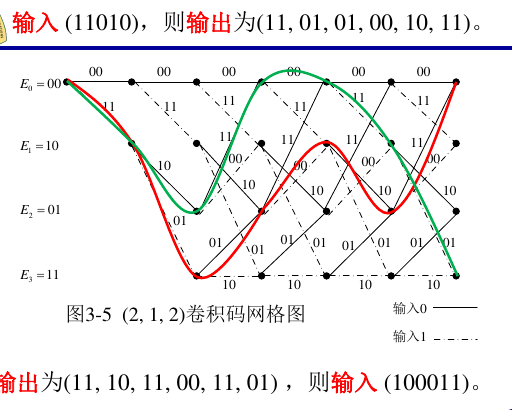
\includegraphics[width=0.7\linewidth]{wanggetu.png}
		\caption{}
		\label{fig:}
	\end{figure}
	维比特译码。
	\item [树图]
\end{description}
\subsubsection{卷积码在蜂窝移动通信系统中的应用}
所有分叉后又合并的任一长度路径中的最小距离称为自由距离df,其纠错能力为$ t = \frac{|d_f -1 |}{2} $。\\
在GSM系统中,使用上述两种编码方式,首先使用CRC编码,在对全部比特做卷积编码。\\
半速率信道编码的自由距离大于全速率信道的自有距离(GSM),反向信道编码的自由距离大于正向信道的自由距离(WCDMA),因此反向信道和半速率信道右更强的抗噪声干扰能力。
\subsection{交织编码}
交织编码的作用是改造信道,其实现方式有\textbf{块
交织,帧交织,随机交织,混合交织}等等。将一个有记忆的突发信道改造成一个随机独立的差错信道。在交织和去交织过程中会产生附加
处理时延。它本身并不具备信道编码检、纠错
功能,仅起到信号预处理的作用。\\
几个名词:
\begin{description}
	\item[交织深度
	] 交织前相邻两符号在交织后的间隔距离
	\item[交织宽度:
	] 交织后相邻两符号在交织前的间隔距离
	\item [交织延迟
	]每个符号从交织器输出时相对于输入交
	织器时的时间延迟
	
\end{description}
对于一个m$\times$n的交织阵列,如果按照\textbf{行写入,列写出},那么交织深度为m,交织宽度为n。\\
要求:交织深度大于相干时间---\textbf{时间分集,是一种时间隐分集技术}
\subsubsection{交织的作用}
交织 + 信道编码 <--> 衰落\\
\vspace{1cm}
交织常与重复或信道编码相结合,是一种对
抗突发错误的时间分集形式,信道编码技术更易于纠正随机错误,交织技
术可以在把信道中的突发错误分散成随机错误;
而衰落是移动通信中引发突发错误的主要因素。

\subsection{Turbo码}
Turbo码巧妙地将\textbf{卷积码}和\textbf{随机交织器}相结合,
采用软输入/输出译码器,可以获得接近Shannon编码
定理极限的性能。但因它存在时延,故主要用于\textbf{非实
时的数据通信}中。

\section{扩频通信}
扩频通信是利用与传输数据(信息)\textbf{无关}的扩频
函数对传输信号扩展频谱,在接收机中利用\textbf{相同}的扩
频函数对接收信号进行同步相关接收、解扩及恢复原
始信息。\\
特征:
\begin{itemize}
	\item 传输带宽远大于被传送信息的原始带宽;
	\item 传输带宽主要由扩频函数决定,扩频函数是不
	可预测的伪随机的宽带信号;
	\item 接收端中用与发射端扩频函数同步的副本实现
	相关解扩。
	
\end{itemize}
\subsection{扩频理论依据}
\textbf{香农定理}:在高斯白噪声干扰条件下,设信
号带宽为B(Hz),信道输出信号平均功率为S
(W),输出加性高斯噪声功率为N(W),则该
通信系统的信道容量C(bit/s)为:
\begin{equation}\label{key}
C = Blog_2(1+\frac{S}{N})
\end{equation}
说明:
\begin{itemize}
	\item 只要信源的信息传输速率Ri小于等于信道容量,即Ri  C,
	则总可以找到一种编码方式实现信号的无差错传输;
	\item 若传输速率大于信道容量,则不可能实现信号的无差错传
	输。
\end{itemize}
扩频信号频谱增加带宽可以换取信噪比的降
低,从而提高了通信的抗干扰能力,实现强干
扰环境下可靠安全的信息传输。\\
两个重要的结论:
\begin{itemize}
	\item 扩频信号频谱增加带宽可以换取信噪比的降
	低,从而提高了通信的抗干扰能力,实现强干
	扰环境下可靠安全的信息传输。
	\item 如果信号的总能量不变,则频谱的展宽势
	必使各谱成分的幅度下降,即功率谱密度降低。
	
\end{itemize}
\subsection{主要工作方式}
\begin{itemize}
	\item 直接序列扩频
	\item 跳变频率扩频
	\item 跳变时间扩频
	\item 宽带线性调频
	\item 混合方式
\end{itemize}
\subsection{主要性能参数}
\subsubsection{扩频处理增益}
\begin{equation}\label{key}
G_p = \frac{SNR_{out}}{SNR_{in}} =10log\frac{SNR_{out}}{SNR_{in}} (db)=  10log\frac{B_{\text{扩频后}}}{B_{\text{扩频前}}} =10log \frac{R_c(\text{伪随机序列发送速率})}{R_b(\text{基带速率})}
\end{equation}
$ G_p $表示了信噪比的改善程度
\subsubsection{干扰容限
}
在保证系统正常工作的条件下
(系统输出信噪比一定),接收机能够承受的干扰信
号比有用信号高出的分贝(dB)数,用M表示,其数学
式为:
\begin{equation}\label{key}
M = G_p - [L_s + (\frac{S}{N}_{out})]dB
\end{equation}
$ L_s $路径传输损耗。\\
干扰容限反映了扩展频谱系统接收机能在多大干
扰环境下正常工作的能力和可能抵抗极限干扰的强度。\\
例:
个扩频系统的处理增益为35dB。要求系
统在误码率小于l0-5时,信息数据解调的最小的
输出信噪比(S/N)out<10dB,系统内部损耗Ls=
3dB,则系统的干扰容限为:
\begin{equation}\label{key}
M = 35 - (3+10) = 22db
\end{equation}
所以系统能够接受,干扰输入电平比扩频信号功率电平高22dB的范围内工作,即接收端输入SNR$\ge$-22dB。
\begin{align*}\label{key}
10logN &- 10logS  \le 22	\\
10logS & \ge 10logN - 22 
\end{align*}
\text{噪声最小为0,所以扩频信号功率电平大于-22dB}
\subsection{伪随机序列
}
为伪噪声序列(PN序列):重复产生和处理,具有\textbf{随机}序列基本特性的\textbf{确定}序列。\\
用作地址码时,要求\textbf{尖锐的自相关,小的互相关}。

\subsubsection{m序列}
最长线性反馈移位寄存器序列,m序列。\\
特征多项式:
\begin{equation}\label{key}
f(x) =  \sum_{r = 0}^{m} = C_rx^r,\text{其中}C_0 = 1,C_m = 1。
\end{equation}
\begin{itemize}
	\item 序列是由多级移位寄存器或其他延迟元件通过线
	性反馈产生的最长的码序列。
	\item 在二进制移位寄存器发生器中,若n为级数,则所
	能产生的最大长度的码序列为$ N=2^n-1 $位,其中等于$ 2^n-1 $的即为m序列。
	\item m序列发生器中,并不是任何抽头组合都能产生m
	序列,需要由本原多项式生成。
\end{itemize}
\textbf{性质:}
\begin{description}
	\item[均衡特性] 在m序列中一个周期内“1”的
	数目比“0”的数目多 1位;
	\item[移位相加性] m序列和其位移序列模2加后仍为m序列
	\item[m序列相关特性] $ R_{a,b}(n) = \frac{A-D}{A+D} $A为相同位数,D为不同位数。\\其自相关函数可表示为
\[ 	 R_{a,a}(n)= \begin{cases}
		1,n=lN\\
		-1/N,其余n
	\end{cases} \]
\end{description}
\textbf{m序列的功率谱:}\\
功率谱具有抽样函数的$ Sa^2(x) $包络,其带宽取决于码元长度。

\subsubsection{Gold码}
性质:
\begin{itemize}
	\item 长度为N的一个优选对可以构成N个Gold码,
	这N个Gold码加上m1和m2,共\textbf{N+2}个码。它们之中
	任何两个码的周期性互相关函数也是三值函数(优选对的性质,即满足优选对的序列,其平移相加后的自相关函数最多有3个值)
	\item  Gold码的个数比m序列数多得多。1对m级移位寄存器m序列,其gold码个数为$ N = 2^m-1 + 2 $。
	\item Gold码的\textbf{周期性自相关函数,自身与自身,自身与本gold码组的其他值}也是三值函数。同
	一优选对产生的Gold码的周期性互相关函数为三值
	函数;同长度的不同优选对产生的Gold码的周期性
	互相关函数不是三值函数;
	\item  Gold序列的互相关峰值、旁瓣与主瓣之比都比
	m序列小得多。\textbf{下行链路}采用gold码\textbf{区分小区和用户,}上行链路用gold码\textbf{区分用户}。
\end{itemize}
\subsubsubsection{Walsh(沃尔什)函数
}
沃尔什函数集是完备的非正弦型正交函
数集,在IS-95CDMA蜂窝移动通信系
统中应用了64阶沃尔什序列\\
哈达玛(Hadamard)矩阵
\[H_{2N} \begin{bmatrix}
	H_{N} & H_{N} \\ 
	H_{N} & -H_{N}
\end{bmatrix}  \]
其中最低阶(2阶的哈达吗矩阵)为:
\[ 
\begin{bmatrix}
1 & 1 \\ 
1 & -1
\end{bmatrix} 
 \]
 任意两行(码字)都是正交的。\\
 
 缺点:
 \begin{itemize}
 	\item Walsh序列的自相关特性不很理想
 	\item 频谱的旁瓣值较大,不利于系统的同步捕
 	获,而且容易产生假同步。
 	\item Walsh码的各码组由于所占频谱带宽不同等
 	原因, 因而不能作为扩频码。
 \end{itemize}
\subsubsection{OVSF码}
为了保证可变扩频码的不同周期长度Walsh码的
正交性,必须满足哈夫曼码在树图上的非延长特性:某一节点的短Walsh码被采用作为扩频正交码以后,
这个节点延长出去的所有树枝上的长Walsh码将不能
再被采用作为扩频正交码。\\
\textbf{速率越高,扩
	频周期越短,频周期越长,扩频比越大。
}\\
按照非延长码规律选取的码组是不等长的正交
码组:
将短码复制(相当与速率高,带宽长,所以将码进行了复制),和最长码一样长。这样,任意两个码都是正交的。
\begin{figure}[H]
	\centering
	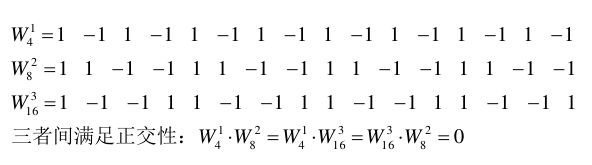
\includegraphics[width=0.7\linewidth]{figures/OVSP}
	\caption{}
	\label{fig:ovsp}
\end{figure}
\subsubsection{地址码}
\begin{itemize}
	\item 区分用户:gold和m
	\item 区分基站:gold
	\item 区分信道:walsh和ovsf
\end{itemize}
\subsection{直接扩频}
扩频:将原始信号于扩频码相乘。\textbf{信号功率下降到原来的1/N}
\begin{figure}[H]
	\centering
	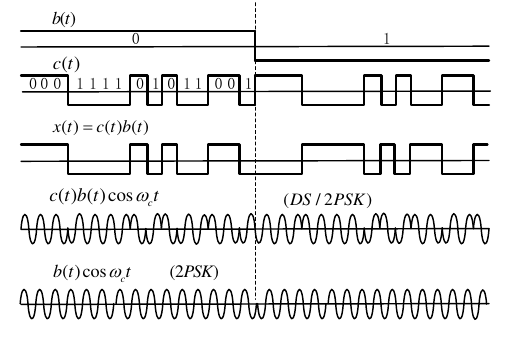
\includegraphics[width=0.7\linewidth]{figures/zhijiekuopin.png}
	\caption{直接扩频}
\end{figure}
\begin{figure}[H]
	\centering
	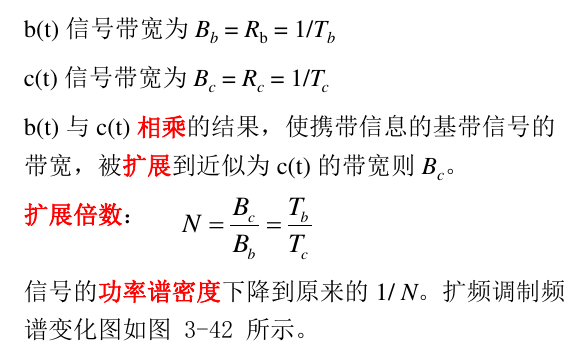
\includegraphics[width=0.7\linewidth]{figures/zhijiekuopin2.png}
	\caption{text}
\end{figure}
解扩:乘以相对应的PN码,还原。
\begin{figure}[H]
	\centering
	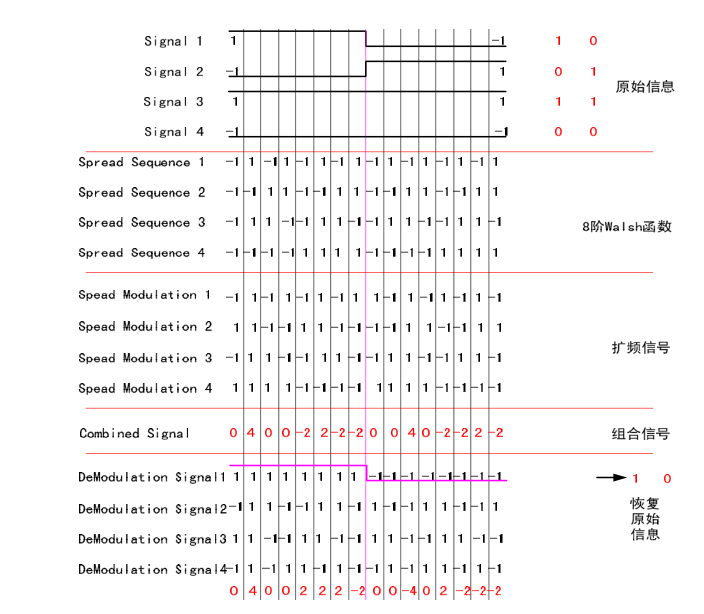
\includegraphics[width=0.9\linewidth]{figures/screenshot002}
	\caption{}
	\label{fig:screenshot002}
\end{figure}
解调方式两种:
\begin{enumerate}
	\item 将Combined信号分别乘上各扩频信号即可得到各路信号。(分离)。适用\textbf{已同步}。
	\item 将扩频信号i分别乘上各扩频信号,得到自相关性强的即为原信号,抖动信号则不是原始信号,适用\textbf{非同步}。
\end{enumerate}
\subsubsection{直接扩频的抗干扰能力}
扩频信号的重要特点:\textbf{抗窄带干扰能力强}
设i(t )为一窄带干扰信号,其频率接近信号的载波频率。
解扩后最终扩频系统的输出干扰功率是输入干扰功率的
1/N ,即扩频系统的处理增益为$ Gp = P_i/P_o = T_b /T_c = N $

\begin{figure}[htbp]
	\centering
	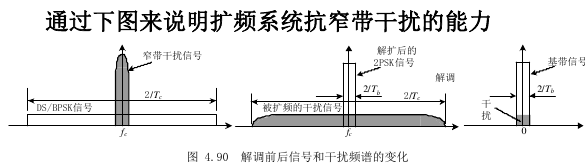
\includegraphics[width=0.9\linewidth]{figures/kangzaidainengli.png}
	\caption{}
	\label{fig:}
\end{figure}
扩频信号对窄带干扰的抑制作用在于接收机
对信号的解扩的同时,对干扰信号的扩频,这降
低了干扰信号的功率谱密度。\\

\section{RAKE接收机}
 利用扩频码的良好自相关特性可以很好地
抑制多径传输带来的干扰 ,当\textbf{多径时延大于扩频码的码片}(时间分集)
的时候 。这些信号 都携带 相同 的
信息 , 利用这些能量 , 则可以
变害为利 , 改善接收信号的质量 
\subsubsection{抗多径干扰}
\begin{itemize}
	\item 利用PN尖锐的自相关特性,很高的码片速率。
	\item  有效抑制与 PN 序列不同步的多径信号分量的干扰
\end{itemize}
\subsubsection{接收方式比较}
\begin{figure}[htbp]
	\centering
	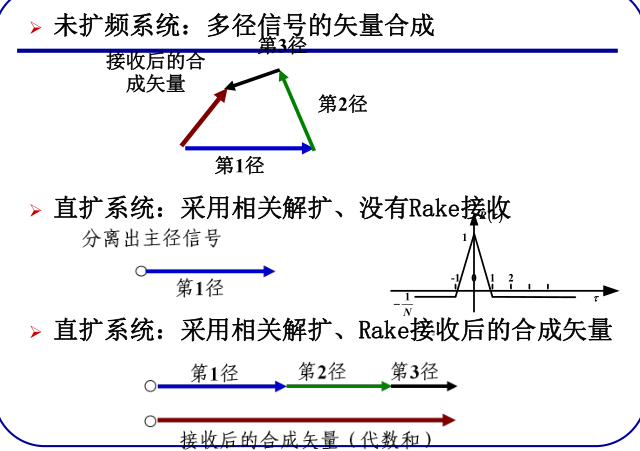
\includegraphics[width=0.7\linewidth]{figures/screenshot001}
	\caption{}
	\label{fig:screenshot001}
\end{figure}
\subsubsection{RAKE接收实现方式}
利用扩频信号设计将各条信号进行\textbf{分离(码片速率小于多径时延差)}。再利用RAKE接收将分离的各条路径信号\textbf{相位校准、幅度加权},将矢量和变为代数和。\\
RAKE接收的本质:时间分集(多径产生时延差)、多径分集、频率分集(扩频带宽远大于相关带宽)。
\section{跳频扩频通信系统}
本质是频率分集。依靠“躲避”来提升抗干扰能力。抗多径、抗同频道干扰、抗衰落。
